A partir de los requisitos especificados, se elaboro la especificacion de requisitos funcionales (SRP), la cual fue estructurada mediante casos de uso y tomando como referencia los lineamientos de la norma IEEE 29148 para la elaboracion de los mismos. El sistema contempla dos actores principales, el administrados y el personal de inventario. El administrador es el tipo de usuario que mas privilegios tiene, es responsable de cargar el historial de consumo e iniciar el procesamiento y gestionar las cuentas de los usuarios. Mientras que el personal de inventario solo usa el sistema para consultar las predicciones y, entre otras actividades, gestionar los pedidos sugeridos. La figura debajo representa los casos de uso correspondientes al Administrador:

\begin{figure}[H]
    \centering
    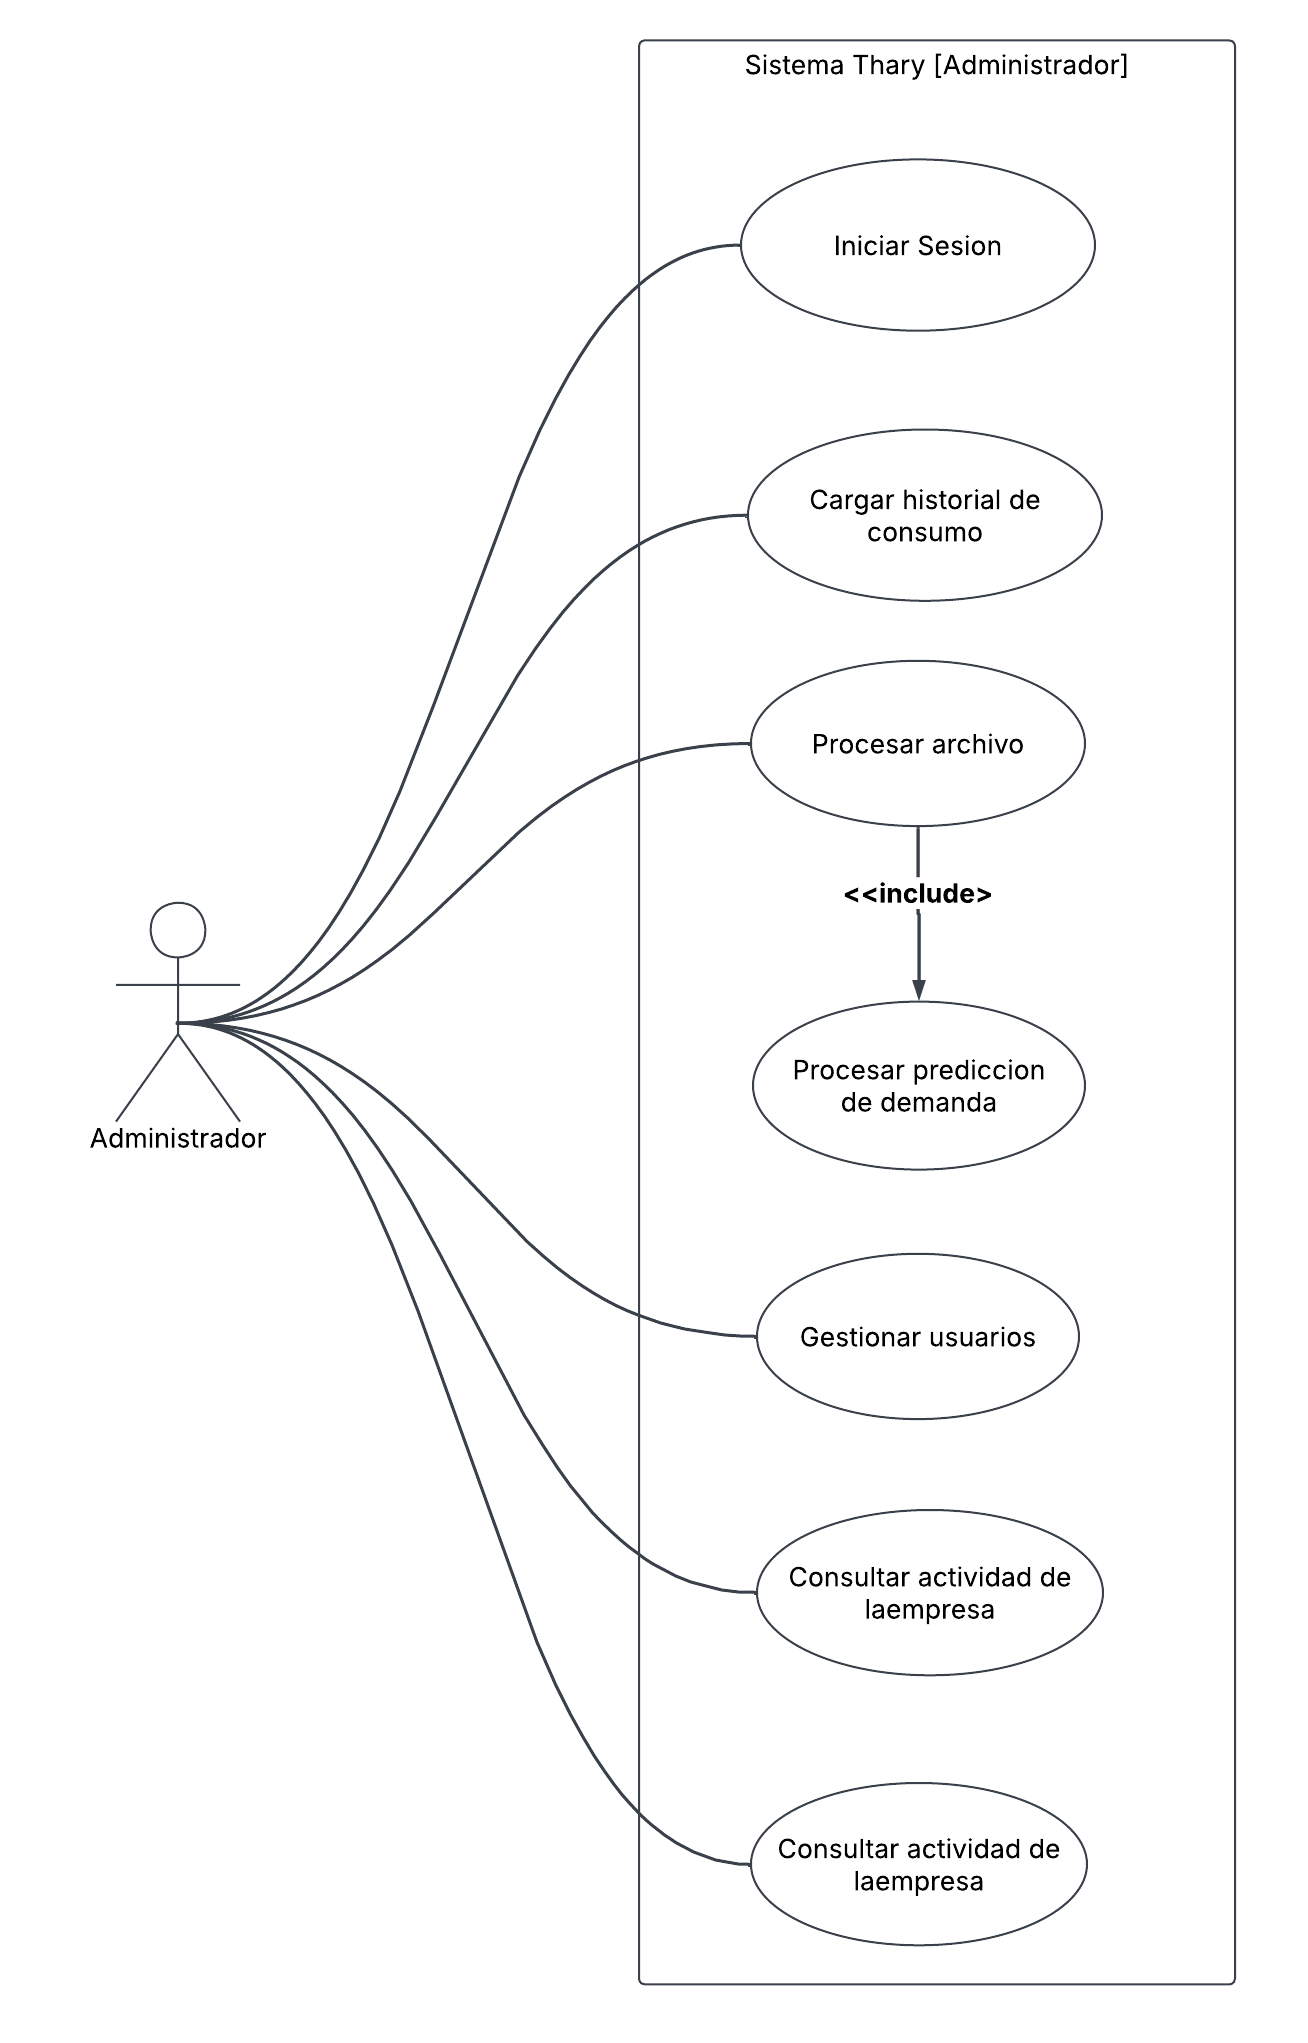
\includegraphics[width=0.48\textwidth]{templatefigures/caso_de_uso_admin.png}
    \caption{Casos de uso del Administrador}
    \label{fig:cu-admin}
\end{figure}

Por su parte, la siguiente figura muestra los casos de uso correspondientes al Personal de Inventario:

\begin{figure}[H]
    \centering
    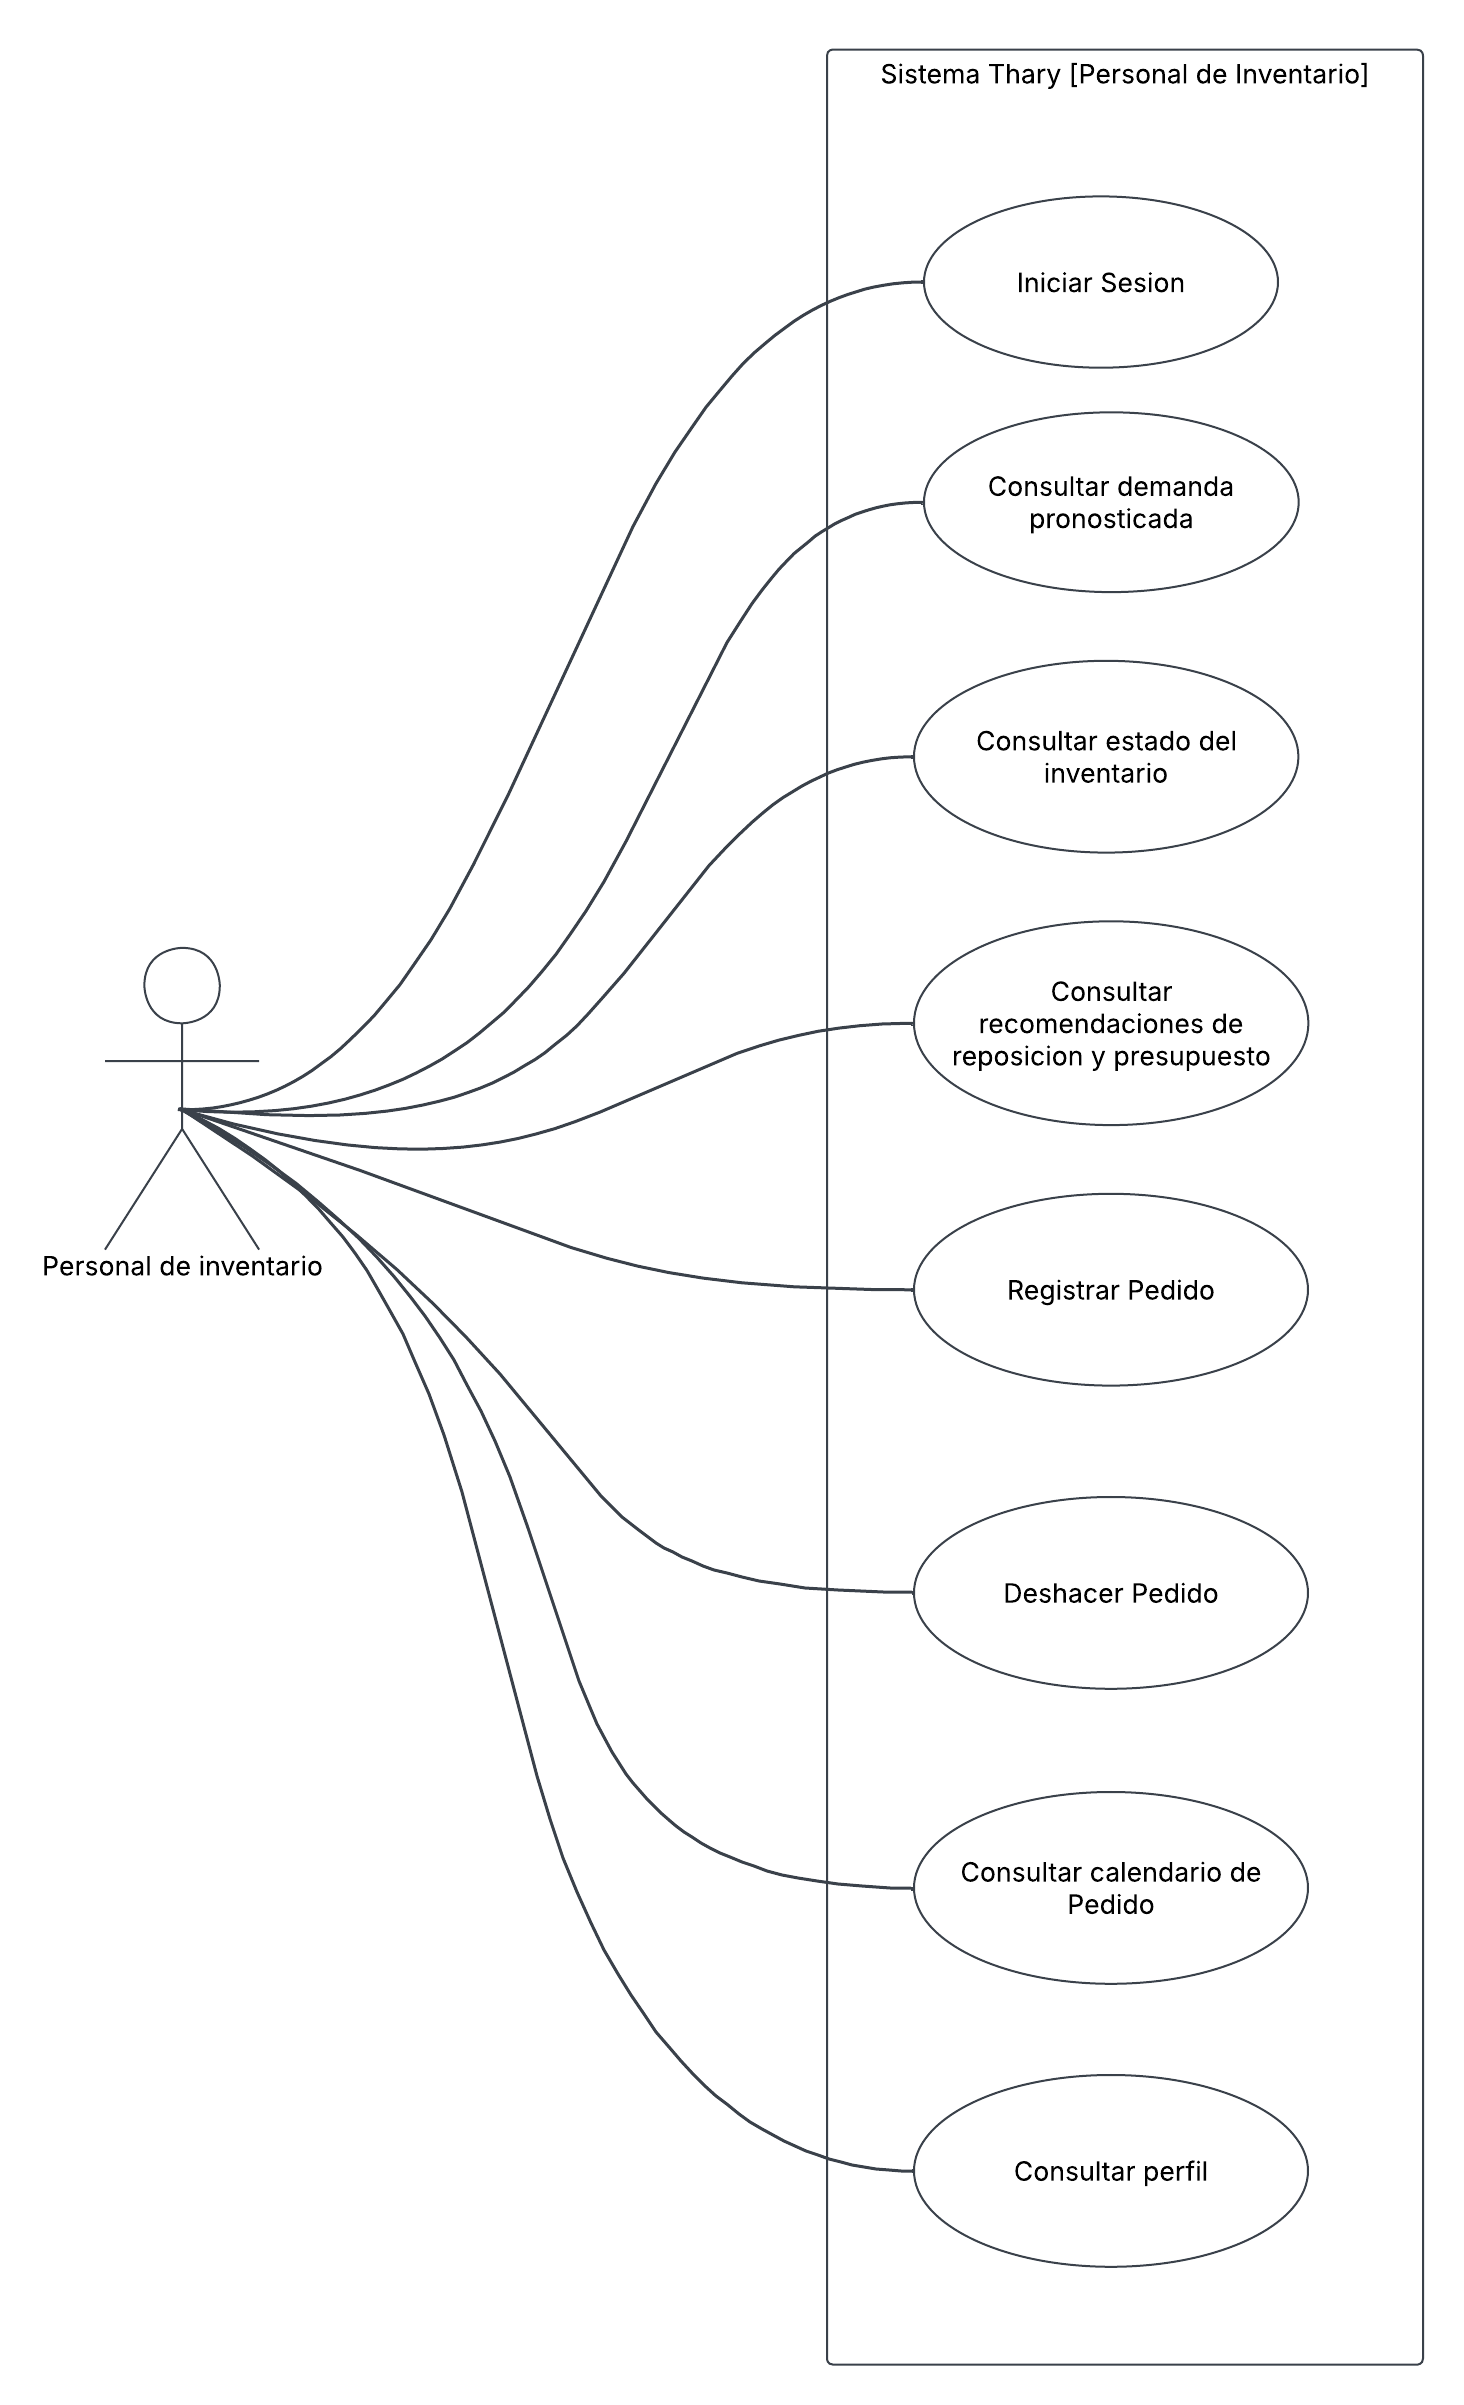
\includegraphics[width=0.48\textwidth]{templatefigures/caso_de_uso_personal.png}
    \caption{Casos de uso del Personal de Inventario}
    \label{fig:cu-personal}
\end{figure}

Como se puede ver en los diagramas, los casos de uso identificados se relacionan con los requisitos funcionales de la siguiente manera:

\begin{table}[H]
\centering
\caption{Trazabilidad entre casos de uso y requisitos funcionales}
\label{tab:trazabilidad_casos_uso}
\begin{tabularx}{\textwidth}{>{\centering\arraybackslash}p{1.2cm} >{\raggedright\arraybackslash}X >{\raggedright\arraybackslash}X >{\centering\arraybackslash}p{3cm}}
\hline
\textbf{ID} & \textbf{Caso de uso} & \textbf{Actor principal} & \textbf{Requisitos relacionados} \\
\hline

CU-01 & Iniciar sesión & Usuario registrado & RF-09 \\

CU-02 & Cargar historial de consumo & Administrador & RF-01, RF-07 \\

CU-03 & Procesar archivo & Administrador & RF-02, RF-07 \\

CU-04 & Consultar demanda pronosticada & Personal de Inventario & RF-02, RF-05 \\

CU-05 & Consultar estado del inventario & Personal de Inventario & RF-04, RF-05 \\

CU-06 & Consultar recomendaciones de reposición y presupuesto & Personal de Inventario & RF-03, RF-05 \\

CU-07 & Registrar pedido & Personal de Inventario & RF-06 \\

CU-08 & Gestionar usuarios & Administrador & RF-08 \\

CU-09 & Deshacer pedido & Personal de Inventario & RF-10 \\

CU-10 & Consultar actividad de la empresa & Administrador & RF-11 \\

CU-11 & Consultar calendario de pedidos & Personal de Inventario & RF-12 \\

CU-12 & Consultar perfil & Usuario registrado & RF-13 \\

\hline
\end{tabularx}
\end{table}


\begin{itemize}

    \item Caso de uso CU-01 (Iniciar sesión (Usuario registrado)): Este caso de uso corresponde al RF-09, y le permite a cualquier usuario registrado ingresar al sistema mediante sus credenciales para acceder a las funcionalidades según su rol.

    \item Caso de uso CU-02 (Cargar historial de consumo (administrador)): Este caso de uso corresponde al RF-01, y permite al administrador seleccionar y cargar el archivo csv con el historial de consumo.

    \item Caso de uso CU-03 (Iniciar procesamiento(Administrador)): Corresponde al requerimiento RF-02, que hace referncia a que una vez cargado el archivo, el administrador debe de seleccionar la opcion "Procesar archivo" para que el sistema inicialice el procesamiento de los datos. 

    \item Caso de uso CU-04 (Consultar demanda pronosticada (Personal de inventario)): Este caso de uso corresponde al RF-02 y al RF-05, y le permite al usuario consultar la demanda mensual estimada para cada producto una vez el archivo ya ha sido procesado.

    \item Caso de uso CU-05 (Consultar estado del inventario (Personal de inventario)): Este caso de uso corresponde a RF-04, que permite al usuario visualizar tanto el inventario disponible como los productos que presentan condiciones de alerta.

    \item Caso de uso CU-06 (Consultar las recomendaciones de reposicion y presupuesto (Personal del inventario)): Corresponde al requisito RF-03, y le permite al usuario consultar las recomendaciones generadas por el sistema y la informacion asociada al presupuesto disponible

    \item Caso de uso CU-07 (Registrar pedido (Personal de inventario)): Este se relaciona directamente con el RF-06, y permite marcar como completado las recomendaciones de pedido generadas por Thary. Los pedidos confirmados quedan registrados con el nombre de la persona que los completa.

    \item Caso de uso CU-08 (Gestionar cuentas de usuario(administrador)): Le permite al administrador el poder crear nuevas cuentas al personal del inventario.
    
    \item Caso de uso CU-09 (Deshacer pedido (Personal de inventario)): Corresponde al RF-10, y le permite al personal de inventario revertir un pedido previamente confirmado, en caso de haberse equivocado o de que la confirmacion ya no sea necesaria.

    \item Caso de uso CU-10 (Consultar actividad de la empresa (Administrador)): Este caso de uso corresponde al RF-11, y le permite al administrador consultar la bitacora completa de acciones realizadas por todos los usuarios de su empresa: carga de archivos, confirmacion o reversion de pedidos, creacion de usuarios, con fines de auditoria.

    \item Caso de uso CU-11 (Consultar calendario de pedidos (Personal de inventario)): Se relaciona con el RF-12, y le permite al usuario visualizar en un calendario las fechas estimadas en las que debe realizarse el pedido de cada producto, segun las recomendaciones generadas por el sistema.

    \item Caso de uso CU-12 (Consultar perfil (Usuario registrado)): Este caso de uso corresponde al RF-13, y le permite a cualquier usuario, sin importar su rol, poder consultar los datos de su propia cuenta y el historial de las acciones que el mismo ha realizado en el sistema.
\end{itemize}

Todos los casos de uso se documentan individualmente en la especificacion SRS presentada en el Anexo A, la cual contempla detalles como objetivo, actor principal, precondiciones y postcondiciones, flujo principales y alternativos.

En cuanto a elementos como las precondiciones, estos se establecen antes de iniciar una funcionalidad, mientras que las postcondiciones describen cual es el estado esperado del sistema al finalizar el proceso, es de esta manera que realizar una correcta especificacion de casos permite establecer una base a la hora de continuar con el proceso de diseño de arquitectura e implementacion de servicios.
